\documentclass[tikz,border=8pt]{standalone}
% Shared look for every TikZ diagram. Load with \input{../../tools/tikz-style.tex}
\usepackage[T1]{fontenc}
\usepackage{lmodern}
\renewcommand{\sfdefault}{lmr}  % diagrams use the same serif as the text
\usetikzlibrary{arrows.meta, positioning, shapes.geometric, calc, fit, backgrounds}
\definecolor{cblue}{HTML}{4C78A8}
\definecolor{corange}{HTML}{F58518}
\definecolor{cgreen}{HTML}{54A24B}
\definecolor{cred}{HTML}{E45756}
\definecolor{cpurple}{HTML}{B279A2}
\definecolor{cgrey}{HTML}{6B6B6B}
\tikzset{
  every picture/.style={font=\sffamily, line width=1.2pt},
  box/.style={draw=#1, fill=#1!12, rounded corners=4pt, align=center, inner sep=7pt, minimum height=1.1cm},
  box/.default=cgrey,
  arrow/.style={-{Stealth[length=3mm]}, draw=cgrey, line width=1.4pt},
  title/.style={font=\sffamily\bfseries\Large},
  note/.style={font=\sffamily\small, text=cgrey, align=center},
}
\AtBeginDocument{\hyphenpenalty=10000 \exhyphenpenalty=10000}

% How AdaBoost and gradient boosting pass the mistakes of one model to the next.
\begin{document}
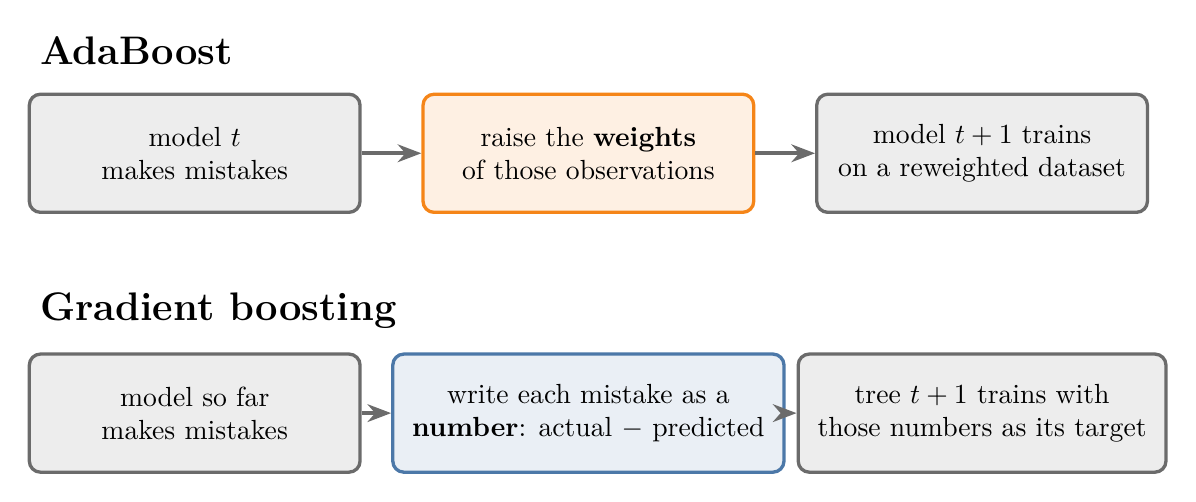
\begin{tikzpicture}[b/.style={box=#1, minimum width=4.2cm, minimum height=1.5cm}]
  \node[title, anchor=west] at (-2.1,1.3) {AdaBoost};
  \node[b=cgrey] (a1) at (0,0) {model $t$\\makes mistakes};
  \node[b=corange] (a2) at (5,0) {raise the \textbf{weights}\\of those observations};
  \node[b=cgrey] (a3) at (10,0) {model $t+1$ trains\\on a reweighted dataset};
  \draw[arrow] (a1) -- (a2); \draw[arrow] (a2) -- (a3);
  \node[title, anchor=west] at (-2.1,-2.0) {Gradient boosting};
  \node[b=cgrey] (g1) at (0,-3.3) {model so far\\makes mistakes};
  \node[b=cblue] (g2) at (5,-3.3) {write each mistake as a\\\textbf{number}: actual $-$ predicted};
  \node[b=cgrey] (g3) at (10,-3.3) {tree $t+1$ trains with\\those numbers as its target};
  \draw[arrow] (g1) -- (g2); \draw[arrow] (g2) -- (g3);
\end{tikzpicture}
\end{document}
